% planner_ablation.tex -- drop-in material for main.tex (2026-09-13, W. Xie / Claude).
%
% Contents
%   1. \subsection{Planner Ablation}\label{sec:planner_ablation}   -- the section
%      main.tex already references (Methods: "We defer the empirical comparison
%      ... to Sec.~\ref{sec:planner_ablation}") but does not yet contain.
%   2. A corrected Table~\ref{tab:planners} (the current one has sigma = 8,
%      10 rollouts, and "elite cov."; none of those is what this fork runs).
%   3. A paragraph for the Discussion on why 33 plans/s suffices, which also
%      explains the 22 Hz desktop failures noted in Task Formulation.
%   4. Feedback on the current draft, as comments at the end of this file.
%
% Every number is from studies/planner_ablation (bench: lean_bench --gains deploy,
% strategy 25, 6 seeds per cell, 33 plans/s unless stated; 1686 runs), page:
% docs/lean/20260911-planner_ablation.html. Figures are in figures/planner/.
%
% Usage: % planner_ablation.tex -- drop-in material for main.tex (2026-09-13, W. Xie / Claude).
%
% Contents
%   1. \subsection{Planner Ablation}\label{sec:planner_ablation}   -- the section
%      main.tex already references (Methods: "We defer the empirical comparison
%      ... to Sec.~\ref{sec:planner_ablation}") but does not yet contain.
%   2. A corrected Table~\ref{tab:planners} (the current one has sigma = 8,
%      10 rollouts, and "elite cov."; none of those is what this fork runs).
%   3. A paragraph for the Discussion on why 33 plans/s suffices, which also
%      explains the 22 Hz desktop failures noted in Task Formulation.
%   4. Feedback on the current draft, as comments at the end of this file.
%
% Every number is from studies/planner_ablation (bench: lean_bench --gains deploy,
% strategy 25, 6 seeds per cell, 33 plans/s unless stated; 1686 runs), page:
% docs/lean/20260911-planner_ablation.html. Figures are in figures/planner/.
%
% Usage: % planner_ablation.tex -- drop-in material for main.tex (2026-09-13, W. Xie / Claude).
%
% Contents
%   1. \subsection{Planner Ablation}\label{sec:planner_ablation}   -- the section
%      main.tex already references (Methods: "We defer the empirical comparison
%      ... to Sec.~\ref{sec:planner_ablation}") but does not yet contain.
%   2. A corrected Table~\ref{tab:planners} (the current one has sigma = 8,
%      10 rollouts, and "elite cov."; none of those is what this fork runs).
%   3. A paragraph for the Discussion on why 33 plans/s suffices, which also
%      explains the 22 Hz desktop failures noted in Task Formulation.
%   4. Feedback on the current draft, as comments at the end of this file.
%
% Every number is from studies/planner_ablation (bench: lean_bench --gains deploy,
% strategy 25, 6 seeds per cell, 33 plans/s unless stated; 1686 runs), page:
% docs/lean/20260911-planner_ablation.html. Figures are in figures/planner/.
%
% Usage: % planner_ablation.tex -- drop-in material for main.tex (2026-09-13, W. Xie / Claude).
%
% Contents
%   1. \subsection{Planner Ablation}\label{sec:planner_ablation}   -- the section
%      main.tex already references (Methods: "We defer the empirical comparison
%      ... to Sec.~\ref{sec:planner_ablation}") but does not yet contain.
%   2. A corrected Table~\ref{tab:planners} (the current one has sigma = 8,
%      10 rollouts, and "elite cov."; none of those is what this fork runs).
%   3. A paragraph for the Discussion on why 33 plans/s suffices, which also
%      explains the 22 Hz desktop failures noted in Task Formulation.
%   4. Feedback on the current draft, as comments at the end of this file.
%
% Every number is from studies/planner_ablation (bench: lean_bench --gains deploy,
% strategy 25, 6 seeds per cell, 33 plans/s unless stated; 1686 runs), page:
% docs/lean/20260911-planner_ablation.html. Figures are in figures/planner/.
%
% Usage: \input{planner_ablation} after the brace-cost ablation, or paste the
% pieces. The section is written to fit in ~0.9 column with one column figure
% (fig_ladder) and one column figure (fig_basin); fig_persist and fig_floor2 are
% offered as appendix figures. Delete the paragraphs marked OPTIONAL to shorten.

%%%%%%%%%%%%%%%%%%%%%%%%%%%%%%%%%%%%%%%%%%%%%%%%%%%%%%%%%%%%%%%%%%%%%%%%%%%%%%%
%% 1. The planner ablation section
%%%%%%%%%%%%%%%%%%%%%%%%%%%%%%%%%%%%%%%%%%%%%%%%%%%%%%%%%%%%%%%%%%%%%%%%%%%%%%%

\begin{figure}[t]
\centering
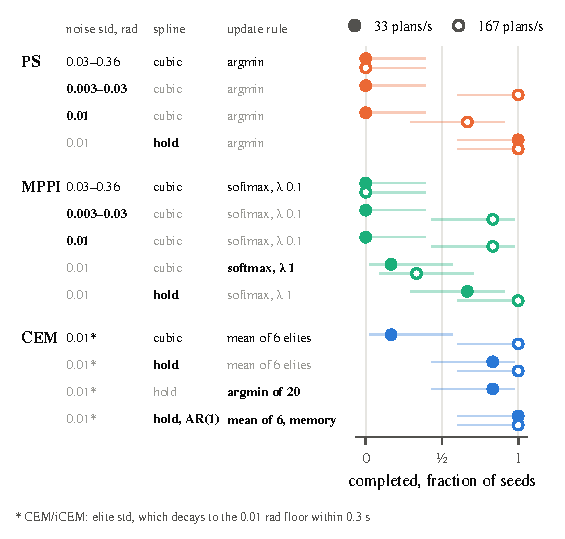
\includegraphics[width=\columnwidth]{figures/planner/fig_ladder.pdf}
\caption{\textbf{From predictive sampling to CEM one component at a time.}
Each row is one planner configuration; in each row the component that changed
from the row above is set in black. Markers show the fraction of six seeds that
completed the lean--reach--recover ladder in simulation at the robot's 33
plans/s (filled) and at 167 plans/s (hollow), with Wilson 95\% intervals.
$0.01^*$: CEM and iCEM sample with the elite standard deviation, which reaches
the $0.01$\,rad floor within $0.3$\,s.}
\label{fig:planner_ladder}
\end{figure}

\subsection{Planner Ablation}\label{sec:planner_ablation}
We compare CEM against predictive sampling (PS) and MPPI on the full ladder
(stand, lean, reach, release, four stand-back rungs) in simulation, on the
robot's joint gains, at the robot's median plan rate of 33 plans/s, six seeds
per configuration (Fig.~\ref{fig:planner_ladder}). As shipped in MJPC, CEM
completes 5/6 and iCEM 6/6; PS and MPPI complete 0/6: PS falls during the initial stand on five of six
seeds (at 4.5--9.9\,s) and collapses onto the table on the sixth, MPPI falls or
collapses before or during the lean on every seed. Two of the three components that differ
between the planners account for the gap, and the update rule
(\textsc{Fold} in Alg.~\ref{alg:skeleton}) is not one of them.

\paragraph{Noise units} CEM and iCEM sample in radians with a $0.01$\,rad
floor. PS and MPPI scale their noise by the actuator control range,
$0.12\times\tfrac12\,\mathrm{ctrlrange}=0.03$--$0.36$\,rad per joint
(median $0.21$\,rad), and drive the position servos with $70$--$130$\,mrad
target steps per plan. Set to $0.01$\,rad in the same units, PS and MPPI
still fail at 33 plans/s (0/6, 1/6) on the cubic spline MJPC's sampling
planner ships with.

\paragraph{Policy representation} With the zero-order hold that CEM and
iCEM hard-code, PS at $0.01$\,rad completes 6/6 and MPPI 4--6/6; with the
cubic spline, CEM itself drops to 1/6. Across twenty spline, knot-count and
noise-colour configurations the separating quantity is how long the sampled
perturbation of the executed action persists in the rollout: every
configuration in which its autocorrelation falls below $0.8$ within
$0.20$\,s completes 0--2/6 and every one that holds it to $0.22$\,s completes
5--6/6, for all four planners (App.~Fig.~\ref{fig:planner_persist}). A hold
with three knots does this by construction ($0.33$\,s); iCEM's AR(1) knot noise
does it by correlation, which is why iCEM alone completes 6/6 with either
spline; white-noise cubic and linear splines do not. At 167 plans/s the
threshold moves below $0.13$\,s and every representation completes.

\paragraph{Update rule} With the hold and $0.01$\,rad every rule completes
the task: argmin (PS, and CEM with one elite) 5--6/6, mean of the $k$ best
5--6/6 for $k\in\{1,2,6,10\}$ and 0/6 for $k=20$ (no selection), softmax
mean 6/6 at $\lambda=0.1$ and 4/6 at $\lambda=1$. The rule decides
sensitivity instead (Fig.~\ref{fig:planner_basin}). Over the twenty
$\sigma\times$plan-rate cells ($\sigma\in\{0.005,\dots,0.05\}$\,rad at 25,
33, 50 and 167 plans/s), CEM completes $\ge 4/6$ in 16, PS with the hold in
12, MPPI with the hold in 10, and PS with its shipped cubic spline in 5; at
33 plans/s CEM's admissible $\sigma$ spans the full tested decade and the
other rules' one octave. The elite mean's random step is $\sigma/\sqrt{k}$
where the argmin's is a full $\sigma$, and that is what lets CEM trade
noise for rate: raising $\sigma$ to $0.02$\,rad takes CEM to 5/6 at
16.7 plans/s and iCEM at $0.03$\,rad to 4/6 at 10 plans/s, where PS and
MPPI gain nothing from the same change.

\begin{figure}[t]
\centering
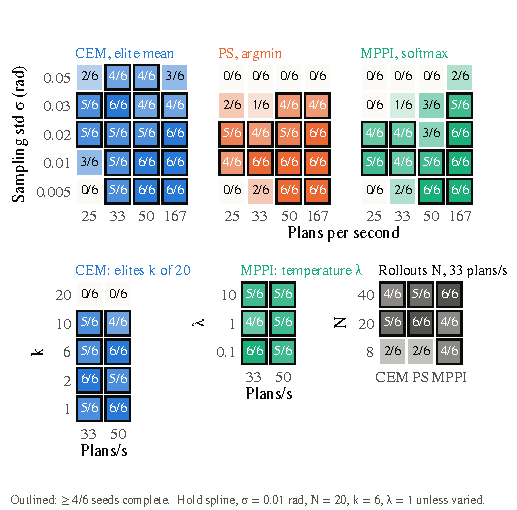
\includegraphics[width=\columnwidth]{figures/planner/fig_basin.pdf}
\caption{\textbf{Sensitivity to configuration.} Completion fraction (6 seeds
per cell) over sampling standard deviation and plan rate for each update
rule at the hold spline; cells at $\ge 4/6$ are outlined. Below: CEM's elite
count, MPPI's temperature, and the rollout count at 33 plans/s.}
\label{fig:planner_basin}
\end{figure}

\paragraph{Plan rate and latency} % OPTIONAL if space is short; the Discussion paragraph below carries the point
At $0.01$\,rad the floor is close to the robot's rate: 25 plans/s completes
1--5/6, 16.7 plans/s 0--1/6, and 10 plans/s 0/6, every failure a backward
fall 2--3\,s into the lean, while the 12\,s stand survives at 5 plans/s. The
executed target step per plan is set by $\sigma$ and the rule, not the rate
(CEM $5$--$8$\,mrad from 167 down to 5 plans/s), so the speed at which the
planner can move its setpoints is step\,$\times$\,rate, and the lean onset
needs $30$--$40$\,mrad/s of directed setpoint motion, which 33 plans/s just
supplies. Latency is a separate quantity: planning
from a state $100$\,ms stale costs nothing at 33 plans/s, $200$\,ms costs
2--5 seeds, and with the state predicted forward as the deploy node does
$200$\,ms costs nothing and $300$\,ms 1--5 seeds. Halving the horizon to
$0.5$\,s completes 0/6, quartering the rollouts 0--2/6, and doubling the
rollout step to $20$\,ms 1--3/6, so the deployed $1$\,s, 20-rollout, $10$\,ms
configuration is close to minimal in every direction but the noise.

\paragraph{Where the rules differ when all complete} % OPTIONAL
The reach rung takes CEM $3.7$\,s, iCEM $4.3$, PS $5.8$ and MPPI
($\lambda=1$) $6.8$\,s, and CEM with six elites braces lightest (peak
$50$\,N, 2\% of the reach on the trunk contact) where PS and MPPI rest on the
table ($138$--$154$\,N, 38--47\%). Under a plant $10\%$ heavier than the
planner's model CEM keeps 3/6 and PS 0/6; under a plant twice as stiff CEM
keeps 6/6, iCEM 4/6, PS 3/6 and MPPI 2/6.

%%%%%%%%%%%%%%%%%%%%%%%%%%%%%%%%%%%%%%%%%%%%%%%%%%%%%%%%%%%%%%%%%%%%%%%%%%%%%%%
%% 2. Replacement for Table~\ref{tab:planners} (the minipage in Methods)
%%%%%%%%%%%%%%%%%%%%%%%%%%%%%%%%%%%%%%%%%%%%%%%%%%%%%%%%%%%%%%%%%%%%%%%%%%%%%%%
% The current table says PS: sigma = 8, argmin, 10 rollouts; CEM: elite cov.
% In this fork every sampling planner reads sampling_trajectories = 20 from
% the task XML, CEM's covariance is diagonal (a per-parameter variance with a
% floor), and PS's sigma is 0.12 x half the control range. Suggested rows:

\refstepcounter{table}
\captionof*{table}{\textbf{Table \thetable.}
How the planners instantiate Alg.~\ref{alg:skeleton} in the deployed
configuration (20 rollouts, 3 spline knots over $1$\,s, a plan every
$30$\,ms). $\sigma$ is the per-knot, per-actuator sampling standard deviation.}
\label{tab:planners}
\centering
\small
\setlength{\tabcolsep}{3pt}
\begin{tabular}{@{}lllll@{}}
\toprule
Planner & \textsc{Center} & \textsc{Spread} & \textsc{Fold} & Spline \\
\midrule
Predictive sampling & $\theta$ (kept as a candidate) & $\sigma = 0.12\cdot\tfrac12\,\mathrm{ctrlrange}$, white & $\arg\min_k J$ & cubic \\
MPPI                & $\theta$ & same as PS & $\sum_k w_k\theta^{(k)},\ w_k\propto e^{-J_k/\lambda}$ & cubic \\
CEM (deployed)      & elite mean & $\max(\text{elite std},\,0.01\,\mathrm{rad})$, diag., white & mean of 6 elites & hold \\
iCEM                & elite mean, 2 elites kept & as CEM, AR(1) across knots ($\alpha=0.7$) & mean of 6 elites & hold \\
\bottomrule
\end{tabular}

%%%%%%%%%%%%%%%%%%%%%%%%%%%%%%%%%%%%%%%%%%%%%%%%%%%%%%%%%%%%%%%%%%%%%%%%%%%%%%%
%% 3. Discussion paragraph: why 33 plans/s is enough
%%%%%%%%%%%%%%%%%%%%%%%%%%%%%%%%%%%%%%%%%%%%%%%%%%%%%%%%%%%%%%%%%%%%%%%%%%%%%%%
% Suggested placement: Sec.~\ref{sec:discussion}, after the first paragraph.
% It also explains the "22 Hz desktop ... increased failure" remark in Task
% Formulation, which the bench reproduces (25 plans/s: CEM 3/6; 16.7: 0/6).

\paragraph{Why 33 plans/s suffices}
Whole-body MPC for locomotion is typically run at 50--100 plans/s over a
300\,Hz tracking controller, because the plan has to re-decide a contact set
every $\approx 0.3$\,s of stance and stabilise an underactuated phase whose
time constant is the pendulum's, $\sqrt{l/g}\approx 0.3$\,s. Supported
reaching has a fixed contact set (double support, then a tripod with the
forearm), a posture the $500$\,Hz joint PD holds between plans, and a single
fast event, the lean onset, that requires the planner to move its position
setpoints at $30$--$40$\,mrad/s (RMS over the 27 joints). A sampling planner moves the setpoints by
roughly one step per plan, so its setpoint speed is step\,$\times$\,rate; at
33 plans/s and $5$--$8$\,mrad per step that is $\approx 190$--$280$\,mrad/s of
executed motion, of which the directed part is enough, and at the 22 plans/s of
the desktop it is not (in simulation CEM completes 3/6 at 25 plans/s and 0/6 at
16.7). The planner here is a setpoint optimiser over a stabilised plant, and
its rate requirement is set by how fast the setpoints have to move, not by the
plant's time constants; a larger sampling step buys back rate, which only the
elite-mean update tolerates.

%%%%%%%%%%%%%%%%%%%%%%%%%%%%%%%%%%%%%%%%%%%%%%%%%%%%%%%%%%%%%%%%%%%%%%%%%%%%%%%
%% Appendix figures (optional)
%%%%%%%%%%%%%%%%%%%%%%%%%%%%%%%%%%%%%%%%%%%%%%%%%%%%%%%%%%%%%%%%%%%%%%%%%%%%%%%

\begin{figure}[t]
\centering
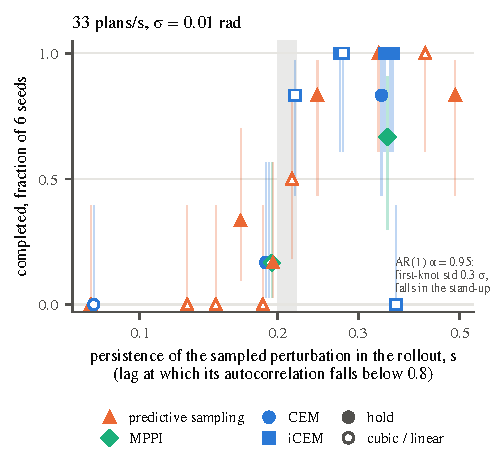
\includegraphics[width=\columnwidth]{figures/planner/fig_persist.pdf}
\caption{\textbf{What the spline changes.} Completion at 33 plans/s and
$0.01$\,rad against the persistence of the sampled perturbation of the
executed action (the lag at which its autocorrelation over the rollout falls
below $0.8$, computed with MJPC's interpolation rules) for twenty spline,
knot-count and noise-colour configurations of PS ($\blacktriangle$), MPPI
($\blacklozenge$), CEM ($\bullet$) and iCEM ($\blacksquare$); hold filled,
cubic or linear hollow. The one point off the step, iCEM with AR(1)
$\alpha=0.95$, fails for amplitude (its first-knot std is $0.3\sigma$).}
\label{fig:planner_persist}
\end{figure}

\begin{figure*}[t]
\centering
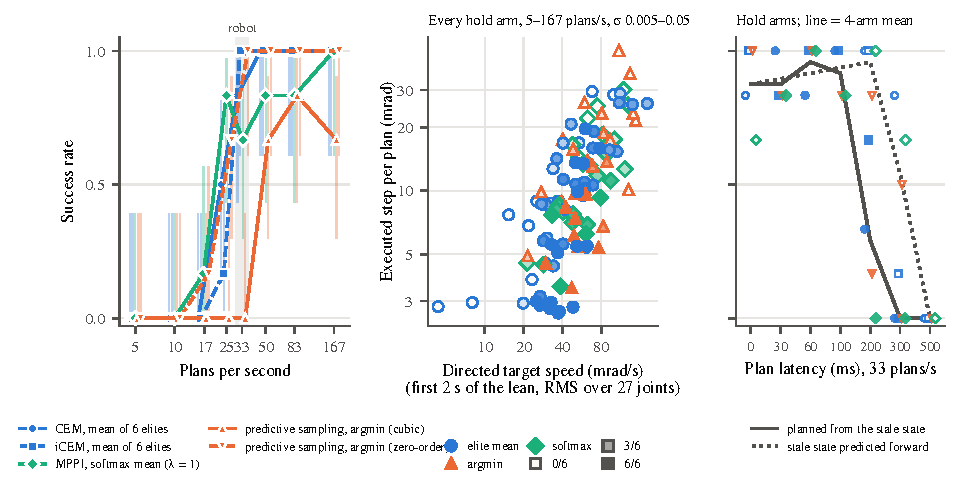
\includegraphics[width=\textwidth]{figures/planner/fig_floor2.pdf}
\caption{\textbf{Plan rate, setpoint speed and latency.} (a) Completion
against plans per second from 5 to 167 for the five update-rule$\times$spline
combinations at $0.01$\,rad; the robot runs at 33. (b) Every hold
configuration at every rate and noise, placed by the directed speed of its
position targets over the first $2$\,s of the lean and by its executed step
per plan; fill is the completion fraction. (c) Completion at 33 plans/s
against plan latency, planned from the stale state (solid) and from the stale
state predicted forward as the deploy node does (dotted).}
\label{fig:planner_floor}
\end{figure*}

%%%%%%%%%%%%%%%%%%%%%%%%%%%%%%%%%%%%%%%%%%%%%%%%%%%%%%%%%%%%%%%%%%%%%%%%%%%%%%%
%% 4. Feedback on main (9).tex (not for the paper; delete)
%%%%%%%%%%%%%%%%%%%%%%%%%%%%%%%%%%%%%%%%%%%%%%%%%%%%%%%%%%%%%%%%%%%%%%%%%%%%%%%
% Dangling / mislabelled references
%  - Methods refers to Sec.~\ref{sec:planner_ablation}; no such label exists.
%    Section 1 above supplies it. The existing "Planner and Cost Ablation"
%    subsection is labelled app:brace_ablation and covers only the brace cost;
%    rename it "Brace-Cost Ablation" and give it its own label.
%  - \label{fig:planners} is a figure with an empty caption
%    (figures/pics/planners_detailed.png); replace with fig_ladder above.
%  - \subsection{Failure Analysis}\label{fig:failure} is referenced as
%    "Sec.~\ref{fig:failure}"; relabel sec:failure.
%  - fig:parameterization (strat11_grid3_topdown_runs.png) has an empty
%    caption; it is the commandability experiment and needs one.
%
% Numbers and consistency
%  - Table tab:planners: "sigma = 8" and "10 rollouts" for PS do not match the
%    deployed task (sampling_exploration 0.12 x half ctrlrange, 20 rollouts);
%    "elite cov." is a diagonal variance with a 0.01 rad floor. See the
%    replacement table.
%  - "The framework uses iLQG ... at 20-50 Hz" (MuJoCo MPC paragraph)
%    describes MJPC's headline planner, not the one deployed here; since the
%    deployed controller is CEM at 33 plans/s, say so in the same sentence or
%    move iLQG to the related-work list.
%  - Task Formulation: "22 Hz planning and increased failure" on the i7 is
%    now explained (Discussion paragraph above): at 0.01 rad the floor is
%    25-33 plans/s.
%  - Leaning, Reaching, and Recovering: "(16/20)$80 \pm 18$\% success (16/20)"
%    duplicates the count; "$100\pm 11$\%" cannot have a symmetric +-11 at
%    100% (Wilson upper bound is 1.0).
%  - Estimation paragraph: "$+267$,mm/min", "$0.48$,m", "$2$,min", "$+210$,mm",
%    "$1$--$2$,mm", "$14$--$47$,mm", "$7$--$10$,mm/s", "$<0.3$,mm" -- the
%    thin-space macro is missing its backslash (should be $267$\,mm/min etc.);
%    same in Target Position Accuracy ("$0.55$,m", "$0.16$,m", "$2.8 \pm 1.3$,cm"
%    ...) and in the fig:target caption.
%  - Abstract says "73% success" for sim-to-real; the body reports 80% on the
%    targeted reach and 73% on max reach -- fine, but say "up to 80%" or name
%    the task in the abstract.
%  - Estimator section: "During such a stand the base genuinely sways, so
%    reported base translation no longer isolates error. Since the base
%    naturally sways during the stand, base translation alone cannot
%    distinguish estimator drift from actual motion." says the same thing
%    twice.
%
% The commandability experiment (Sec. sec:icra, strategy 11)
%  - The bench can give a simulation counterpart on strategy 25's 3x3 target
%    grid (target_col_x / target_col_y numerics) for the four planners; that
%    sweep is running as this file is written (runs/grid_spp15, 3 seeds per
%    cell) and will be reported on the study page. On hardware the natural
%    planner-side statement is that the elite mean's sigma basin (Fig.
%    fig:planner_basin) is what makes one set of weights hold across targets
%    and heights without retuning; the sim grid tests that.
%  - The one model parameter the controller is exposed to is mass (a 10%
%    heavier plant halves completion without gravity feedforward); if the
%    height/target grid carries a payload, say what the payload is relative
%    to the model.
 after the brace-cost ablation, or paste the
% pieces. The section is written to fit in ~0.9 column with one column figure
% (fig_ladder) and one column figure (fig_basin); fig_persist and fig_floor2 are
% offered as appendix figures. Delete the paragraphs marked OPTIONAL to shorten.

%%%%%%%%%%%%%%%%%%%%%%%%%%%%%%%%%%%%%%%%%%%%%%%%%%%%%%%%%%%%%%%%%%%%%%%%%%%%%%%
%% 1. The planner ablation section
%%%%%%%%%%%%%%%%%%%%%%%%%%%%%%%%%%%%%%%%%%%%%%%%%%%%%%%%%%%%%%%%%%%%%%%%%%%%%%%

\begin{figure}[t]
\centering
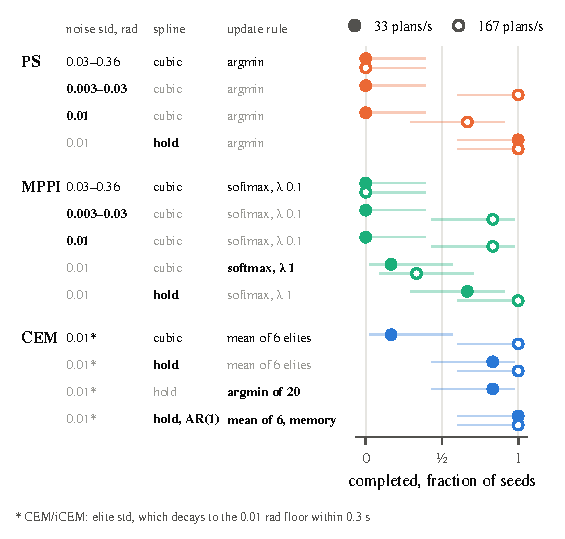
\includegraphics[width=\columnwidth]{figures/planner/fig_ladder.pdf}
\caption{\textbf{From predictive sampling to CEM one component at a time.}
Each row is one planner configuration; in each row the component that changed
from the row above is set in black. Markers show the fraction of six seeds that
completed the lean--reach--recover ladder in simulation at the robot's 33
plans/s (filled) and at 167 plans/s (hollow), with Wilson 95\% intervals.
$0.01^*$: CEM and iCEM sample with the elite standard deviation, which reaches
the $0.01$\,rad floor within $0.3$\,s.}
\label{fig:planner_ladder}
\end{figure}

\subsection{Planner Ablation}\label{sec:planner_ablation}
We compare CEM against predictive sampling (PS) and MPPI on the full ladder
(stand, lean, reach, release, four stand-back rungs) in simulation, on the
robot's joint gains, at the robot's median plan rate of 33 plans/s, six seeds
per configuration (Fig.~\ref{fig:planner_ladder}). As shipped in MJPC, CEM
completes 5/6 and iCEM 6/6; PS and MPPI complete 0/6: PS falls during the initial stand on five of six
seeds (at 4.5--9.9\,s) and collapses onto the table on the sixth, MPPI falls or
collapses before or during the lean on every seed. Two of the three components that differ
between the planners account for the gap, and the update rule
(\textsc{Fold} in Alg.~\ref{alg:skeleton}) is not one of them.

\paragraph{Noise units} CEM and iCEM sample in radians with a $0.01$\,rad
floor. PS and MPPI scale their noise by the actuator control range,
$0.12\times\tfrac12\,\mathrm{ctrlrange}=0.03$--$0.36$\,rad per joint
(median $0.21$\,rad), and drive the position servos with $70$--$130$\,mrad
target steps per plan. Set to $0.01$\,rad in the same units, PS and MPPI
still fail at 33 plans/s (0/6, 1/6) on the cubic spline MJPC's sampling
planner ships with.

\paragraph{Policy representation} With the zero-order hold that CEM and
iCEM hard-code, PS at $0.01$\,rad completes 6/6 and MPPI 4--6/6; with the
cubic spline, CEM itself drops to 1/6. Across twenty spline, knot-count and
noise-colour configurations the separating quantity is how long the sampled
perturbation of the executed action persists in the rollout: every
configuration in which its autocorrelation falls below $0.8$ within
$0.20$\,s completes 0--2/6 and every one that holds it to $0.22$\,s completes
5--6/6, for all four planners (App.~Fig.~\ref{fig:planner_persist}). A hold
with three knots does this by construction ($0.33$\,s); iCEM's AR(1) knot noise
does it by correlation, which is why iCEM alone completes 6/6 with either
spline; white-noise cubic and linear splines do not. At 167 plans/s the
threshold moves below $0.13$\,s and every representation completes.

\paragraph{Update rule} With the hold and $0.01$\,rad every rule completes
the task: argmin (PS, and CEM with one elite) 5--6/6, mean of the $k$ best
5--6/6 for $k\in\{1,2,6,10\}$ and 0/6 for $k=20$ (no selection), softmax
mean 6/6 at $\lambda=0.1$ and 4/6 at $\lambda=1$. The rule decides
sensitivity instead (Fig.~\ref{fig:planner_basin}). Over the twenty
$\sigma\times$plan-rate cells ($\sigma\in\{0.005,\dots,0.05\}$\,rad at 25,
33, 50 and 167 plans/s), CEM completes $\ge 4/6$ in 16, PS with the hold in
12, MPPI with the hold in 10, and PS with its shipped cubic spline in 5; at
33 plans/s CEM's admissible $\sigma$ spans the full tested decade and the
other rules' one octave. The elite mean's random step is $\sigma/\sqrt{k}$
where the argmin's is a full $\sigma$, and that is what lets CEM trade
noise for rate: raising $\sigma$ to $0.02$\,rad takes CEM to 5/6 at
16.7 plans/s and iCEM at $0.03$\,rad to 4/6 at 10 plans/s, where PS and
MPPI gain nothing from the same change.

\begin{figure}[t]
\centering
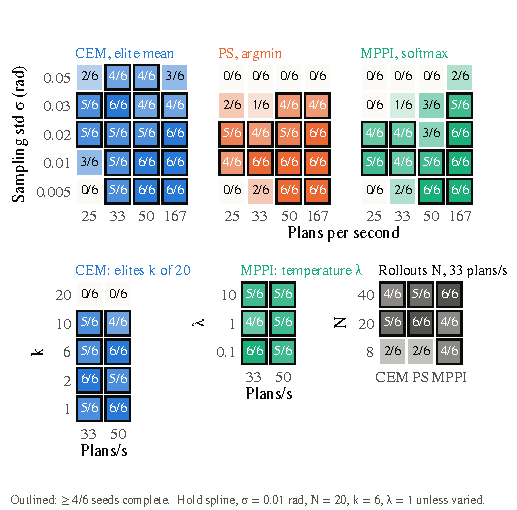
\includegraphics[width=\columnwidth]{figures/planner/fig_basin.pdf}
\caption{\textbf{Sensitivity to configuration.} Completion fraction (6 seeds
per cell) over sampling standard deviation and plan rate for each update
rule at the hold spline; cells at $\ge 4/6$ are outlined. Below: CEM's elite
count, MPPI's temperature, and the rollout count at 33 plans/s.}
\label{fig:planner_basin}
\end{figure}

\paragraph{Plan rate and latency} % OPTIONAL if space is short; the Discussion paragraph below carries the point
At $0.01$\,rad the floor is close to the robot's rate: 25 plans/s completes
1--5/6, 16.7 plans/s 0--1/6, and 10 plans/s 0/6, every failure a backward
fall 2--3\,s into the lean, while the 12\,s stand survives at 5 plans/s. The
executed target step per plan is set by $\sigma$ and the rule, not the rate
(CEM $5$--$8$\,mrad from 167 down to 5 plans/s), so the speed at which the
planner can move its setpoints is step\,$\times$\,rate, and the lean onset
needs $30$--$40$\,mrad/s of directed setpoint motion, which 33 plans/s just
supplies. Latency is a separate quantity: planning
from a state $100$\,ms stale costs nothing at 33 plans/s, $200$\,ms costs
2--5 seeds, and with the state predicted forward as the deploy node does
$200$\,ms costs nothing and $300$\,ms 1--5 seeds. Halving the horizon to
$0.5$\,s completes 0/6, quartering the rollouts 0--2/6, and doubling the
rollout step to $20$\,ms 1--3/6, so the deployed $1$\,s, 20-rollout, $10$\,ms
configuration is close to minimal in every direction but the noise.

\paragraph{Where the rules differ when all complete} % OPTIONAL
The reach rung takes CEM $3.7$\,s, iCEM $4.3$, PS $5.8$ and MPPI
($\lambda=1$) $6.8$\,s, and CEM with six elites braces lightest (peak
$50$\,N, 2\% of the reach on the trunk contact) where PS and MPPI rest on the
table ($138$--$154$\,N, 38--47\%). Under a plant $10\%$ heavier than the
planner's model CEM keeps 3/6 and PS 0/6; under a plant twice as stiff CEM
keeps 6/6, iCEM 4/6, PS 3/6 and MPPI 2/6.

%%%%%%%%%%%%%%%%%%%%%%%%%%%%%%%%%%%%%%%%%%%%%%%%%%%%%%%%%%%%%%%%%%%%%%%%%%%%%%%
%% 2. Replacement for Table~\ref{tab:planners} (the minipage in Methods)
%%%%%%%%%%%%%%%%%%%%%%%%%%%%%%%%%%%%%%%%%%%%%%%%%%%%%%%%%%%%%%%%%%%%%%%%%%%%%%%
% The current table says PS: sigma = 8, argmin, 10 rollouts; CEM: elite cov.
% In this fork every sampling planner reads sampling_trajectories = 20 from
% the task XML, CEM's covariance is diagonal (a per-parameter variance with a
% floor), and PS's sigma is 0.12 x half the control range. Suggested rows:

\refstepcounter{table}
\captionof*{table}{\textbf{Table \thetable.}
How the planners instantiate Alg.~\ref{alg:skeleton} in the deployed
configuration (20 rollouts, 3 spline knots over $1$\,s, a plan every
$30$\,ms). $\sigma$ is the per-knot, per-actuator sampling standard deviation.}
\label{tab:planners}
\centering
\small
\setlength{\tabcolsep}{3pt}
\begin{tabular}{@{}lllll@{}}
\toprule
Planner & \textsc{Center} & \textsc{Spread} & \textsc{Fold} & Spline \\
\midrule
Predictive sampling & $\theta$ (kept as a candidate) & $\sigma = 0.12\cdot\tfrac12\,\mathrm{ctrlrange}$, white & $\arg\min_k J$ & cubic \\
MPPI                & $\theta$ & same as PS & $\sum_k w_k\theta^{(k)},\ w_k\propto e^{-J_k/\lambda}$ & cubic \\
CEM (deployed)      & elite mean & $\max(\text{elite std},\,0.01\,\mathrm{rad})$, diag., white & mean of 6 elites & hold \\
iCEM                & elite mean, 2 elites kept & as CEM, AR(1) across knots ($\alpha=0.7$) & mean of 6 elites & hold \\
\bottomrule
\end{tabular}

%%%%%%%%%%%%%%%%%%%%%%%%%%%%%%%%%%%%%%%%%%%%%%%%%%%%%%%%%%%%%%%%%%%%%%%%%%%%%%%
%% 3. Discussion paragraph: why 33 plans/s is enough
%%%%%%%%%%%%%%%%%%%%%%%%%%%%%%%%%%%%%%%%%%%%%%%%%%%%%%%%%%%%%%%%%%%%%%%%%%%%%%%
% Suggested placement: Sec.~\ref{sec:discussion}, after the first paragraph.
% It also explains the "22 Hz desktop ... increased failure" remark in Task
% Formulation, which the bench reproduces (25 plans/s: CEM 3/6; 16.7: 0/6).

\paragraph{Why 33 plans/s suffices}
Whole-body MPC for locomotion is typically run at 50--100 plans/s over a
300\,Hz tracking controller, because the plan has to re-decide a contact set
every $\approx 0.3$\,s of stance and stabilise an underactuated phase whose
time constant is the pendulum's, $\sqrt{l/g}\approx 0.3$\,s. Supported
reaching has a fixed contact set (double support, then a tripod with the
forearm), a posture the $500$\,Hz joint PD holds between plans, and a single
fast event, the lean onset, that requires the planner to move its position
setpoints at $30$--$40$\,mrad/s (RMS over the 27 joints). A sampling planner moves the setpoints by
roughly one step per plan, so its setpoint speed is step\,$\times$\,rate; at
33 plans/s and $5$--$8$\,mrad per step that is $\approx 190$--$280$\,mrad/s of
executed motion, of which the directed part is enough, and at the 22 plans/s of
the desktop it is not (in simulation CEM completes 3/6 at 25 plans/s and 0/6 at
16.7). The planner here is a setpoint optimiser over a stabilised plant, and
its rate requirement is set by how fast the setpoints have to move, not by the
plant's time constants; a larger sampling step buys back rate, which only the
elite-mean update tolerates.

%%%%%%%%%%%%%%%%%%%%%%%%%%%%%%%%%%%%%%%%%%%%%%%%%%%%%%%%%%%%%%%%%%%%%%%%%%%%%%%
%% Appendix figures (optional)
%%%%%%%%%%%%%%%%%%%%%%%%%%%%%%%%%%%%%%%%%%%%%%%%%%%%%%%%%%%%%%%%%%%%%%%%%%%%%%%

\begin{figure}[t]
\centering
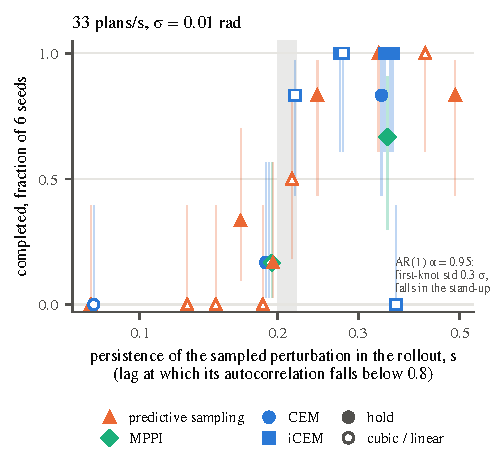
\includegraphics[width=\columnwidth]{figures/planner/fig_persist.pdf}
\caption{\textbf{What the spline changes.} Completion at 33 plans/s and
$0.01$\,rad against the persistence of the sampled perturbation of the
executed action (the lag at which its autocorrelation over the rollout falls
below $0.8$, computed with MJPC's interpolation rules) for twenty spline,
knot-count and noise-colour configurations of PS ($\blacktriangle$), MPPI
($\blacklozenge$), CEM ($\bullet$) and iCEM ($\blacksquare$); hold filled,
cubic or linear hollow. The one point off the step, iCEM with AR(1)
$\alpha=0.95$, fails for amplitude (its first-knot std is $0.3\sigma$).}
\label{fig:planner_persist}
\end{figure}

\begin{figure*}[t]
\centering
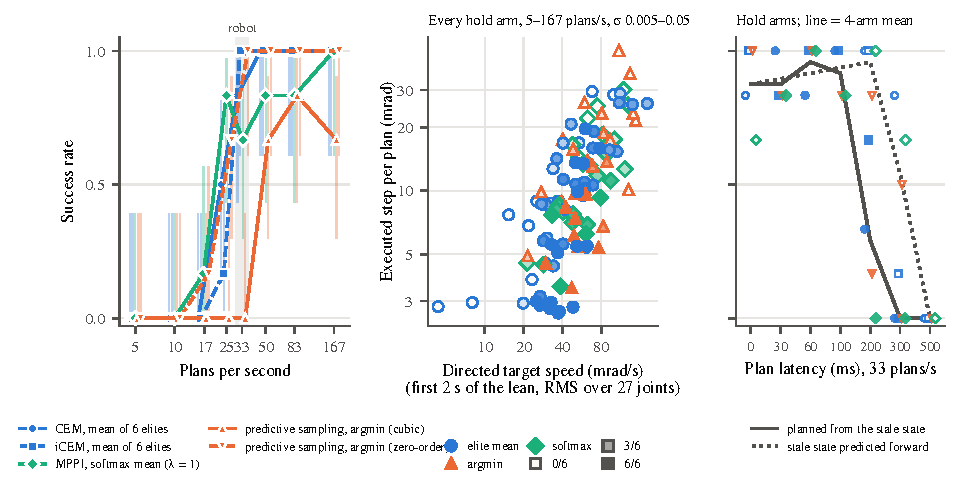
\includegraphics[width=\textwidth]{figures/planner/fig_floor2.pdf}
\caption{\textbf{Plan rate, setpoint speed and latency.} (a) Completion
against plans per second from 5 to 167 for the five update-rule$\times$spline
combinations at $0.01$\,rad; the robot runs at 33. (b) Every hold
configuration at every rate and noise, placed by the directed speed of its
position targets over the first $2$\,s of the lean and by its executed step
per plan; fill is the completion fraction. (c) Completion at 33 plans/s
against plan latency, planned from the stale state (solid) and from the stale
state predicted forward as the deploy node does (dotted).}
\label{fig:planner_floor}
\end{figure*}

%%%%%%%%%%%%%%%%%%%%%%%%%%%%%%%%%%%%%%%%%%%%%%%%%%%%%%%%%%%%%%%%%%%%%%%%%%%%%%%
%% 4. Feedback on main (9).tex (not for the paper; delete)
%%%%%%%%%%%%%%%%%%%%%%%%%%%%%%%%%%%%%%%%%%%%%%%%%%%%%%%%%%%%%%%%%%%%%%%%%%%%%%%
% Dangling / mislabelled references
%  - Methods refers to Sec.~\ref{sec:planner_ablation}; no such label exists.
%    Section 1 above supplies it. The existing "Planner and Cost Ablation"
%    subsection is labelled app:brace_ablation and covers only the brace cost;
%    rename it "Brace-Cost Ablation" and give it its own label.
%  - \label{fig:planners} is a figure with an empty caption
%    (figures/pics/planners_detailed.png); replace with fig_ladder above.
%  - \subsection{Failure Analysis}\label{fig:failure} is referenced as
%    "Sec.~\ref{fig:failure}"; relabel sec:failure.
%  - fig:parameterization (strat11_grid3_topdown_runs.png) has an empty
%    caption; it is the commandability experiment and needs one.
%
% Numbers and consistency
%  - Table tab:planners: "sigma = 8" and "10 rollouts" for PS do not match the
%    deployed task (sampling_exploration 0.12 x half ctrlrange, 20 rollouts);
%    "elite cov." is a diagonal variance with a 0.01 rad floor. See the
%    replacement table.
%  - "The framework uses iLQG ... at 20-50 Hz" (MuJoCo MPC paragraph)
%    describes MJPC's headline planner, not the one deployed here; since the
%    deployed controller is CEM at 33 plans/s, say so in the same sentence or
%    move iLQG to the related-work list.
%  - Task Formulation: "22 Hz planning and increased failure" on the i7 is
%    now explained (Discussion paragraph above): at 0.01 rad the floor is
%    25-33 plans/s.
%  - Leaning, Reaching, and Recovering: "(16/20)$80 \pm 18$\% success (16/20)"
%    duplicates the count; "$100\pm 11$\%" cannot have a symmetric +-11 at
%    100% (Wilson upper bound is 1.0).
%  - Estimation paragraph: "$+267$,mm/min", "$0.48$,m", "$2$,min", "$+210$,mm",
%    "$1$--$2$,mm", "$14$--$47$,mm", "$7$--$10$,mm/s", "$<0.3$,mm" -- the
%    thin-space macro is missing its backslash (should be $267$\,mm/min etc.);
%    same in Target Position Accuracy ("$0.55$,m", "$0.16$,m", "$2.8 \pm 1.3$,cm"
%    ...) and in the fig:target caption.
%  - Abstract says "73% success" for sim-to-real; the body reports 80% on the
%    targeted reach and 73% on max reach -- fine, but say "up to 80%" or name
%    the task in the abstract.
%  - Estimator section: "During such a stand the base genuinely sways, so
%    reported base translation no longer isolates error. Since the base
%    naturally sways during the stand, base translation alone cannot
%    distinguish estimator drift from actual motion." says the same thing
%    twice.
%
% The commandability experiment (Sec. sec:icra, strategy 11)
%  - The bench can give a simulation counterpart on strategy 25's 3x3 target
%    grid (target_col_x / target_col_y numerics) for the four planners; that
%    sweep is running as this file is written (runs/grid_spp15, 3 seeds per
%    cell) and will be reported on the study page. On hardware the natural
%    planner-side statement is that the elite mean's sigma basin (Fig.
%    fig:planner_basin) is what makes one set of weights hold across targets
%    and heights without retuning; the sim grid tests that.
%  - The one model parameter the controller is exposed to is mass (a 10%
%    heavier plant halves completion without gravity feedforward); if the
%    height/target grid carries a payload, say what the payload is relative
%    to the model.
 after the brace-cost ablation, or paste the
% pieces. The section is written to fit in ~0.9 column with one column figure
% (fig_ladder) and one column figure (fig_basin); fig_persist and fig_floor2 are
% offered as appendix figures. Delete the paragraphs marked OPTIONAL to shorten.

%%%%%%%%%%%%%%%%%%%%%%%%%%%%%%%%%%%%%%%%%%%%%%%%%%%%%%%%%%%%%%%%%%%%%%%%%%%%%%%
%% 1. The planner ablation section
%%%%%%%%%%%%%%%%%%%%%%%%%%%%%%%%%%%%%%%%%%%%%%%%%%%%%%%%%%%%%%%%%%%%%%%%%%%%%%%

\begin{figure}[t]
\centering
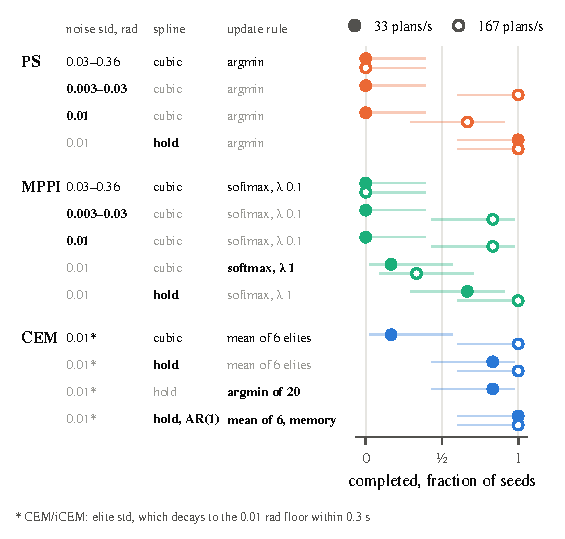
\includegraphics[width=\columnwidth]{figures/planner/fig_ladder.pdf}
\caption{\textbf{From predictive sampling to CEM one component at a time.}
Each row is one planner configuration; in each row the component that changed
from the row above is set in black. Markers show the fraction of six seeds that
completed the lean--reach--recover ladder in simulation at the robot's 33
plans/s (filled) and at 167 plans/s (hollow), with Wilson 95\% intervals.
$0.01^*$: CEM and iCEM sample with the elite standard deviation, which reaches
the $0.01$\,rad floor within $0.3$\,s.}
\label{fig:planner_ladder}
\end{figure}

\subsection{Planner Ablation}\label{sec:planner_ablation}
We compare CEM against predictive sampling (PS) and MPPI on the full ladder
(stand, lean, reach, release, four stand-back rungs) in simulation, on the
robot's joint gains, at the robot's median plan rate of 33 plans/s, six seeds
per configuration (Fig.~\ref{fig:planner_ladder}). As shipped in MJPC, CEM
completes 5/6 and iCEM 6/6; PS and MPPI complete 0/6: PS falls during the initial stand on five of six
seeds (at 4.5--9.9\,s) and collapses onto the table on the sixth, MPPI falls or
collapses before or during the lean on every seed. Two of the three components that differ
between the planners account for the gap, and the update rule
(\textsc{Fold} in Alg.~\ref{alg:skeleton}) is not one of them.

\paragraph{Noise units} CEM and iCEM sample in radians with a $0.01$\,rad
floor. PS and MPPI scale their noise by the actuator control range,
$0.12\times\tfrac12\,\mathrm{ctrlrange}=0.03$--$0.36$\,rad per joint
(median $0.21$\,rad), and drive the position servos with $70$--$130$\,mrad
target steps per plan. Set to $0.01$\,rad in the same units, PS and MPPI
still fail at 33 plans/s (0/6, 1/6) on the cubic spline MJPC's sampling
planner ships with.

\paragraph{Policy representation} With the zero-order hold that CEM and
iCEM hard-code, PS at $0.01$\,rad completes 6/6 and MPPI 4--6/6; with the
cubic spline, CEM itself drops to 1/6. Across twenty spline, knot-count and
noise-colour configurations the separating quantity is how long the sampled
perturbation of the executed action persists in the rollout: every
configuration in which its autocorrelation falls below $0.8$ within
$0.20$\,s completes 0--2/6 and every one that holds it to $0.22$\,s completes
5--6/6, for all four planners (App.~Fig.~\ref{fig:planner_persist}). A hold
with three knots does this by construction ($0.33$\,s); iCEM's AR(1) knot noise
does it by correlation, which is why iCEM alone completes 6/6 with either
spline; white-noise cubic and linear splines do not. At 167 plans/s the
threshold moves below $0.13$\,s and every representation completes.

\paragraph{Update rule} With the hold and $0.01$\,rad every rule completes
the task: argmin (PS, and CEM with one elite) 5--6/6, mean of the $k$ best
5--6/6 for $k\in\{1,2,6,10\}$ and 0/6 for $k=20$ (no selection), softmax
mean 6/6 at $\lambda=0.1$ and 4/6 at $\lambda=1$. The rule decides
sensitivity instead (Fig.~\ref{fig:planner_basin}). Over the twenty
$\sigma\times$plan-rate cells ($\sigma\in\{0.005,\dots,0.05\}$\,rad at 25,
33, 50 and 167 plans/s), CEM completes $\ge 4/6$ in 16, PS with the hold in
12, MPPI with the hold in 10, and PS with its shipped cubic spline in 5; at
33 plans/s CEM's admissible $\sigma$ spans the full tested decade and the
other rules' one octave. The elite mean's random step is $\sigma/\sqrt{k}$
where the argmin's is a full $\sigma$, and that is what lets CEM trade
noise for rate: raising $\sigma$ to $0.02$\,rad takes CEM to 5/6 at
16.7 plans/s and iCEM at $0.03$\,rad to 4/6 at 10 plans/s, where PS and
MPPI gain nothing from the same change.

\begin{figure}[t]
\centering
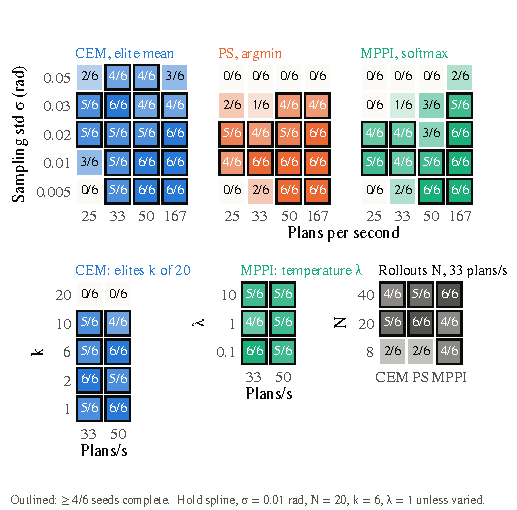
\includegraphics[width=\columnwidth]{figures/planner/fig_basin.pdf}
\caption{\textbf{Sensitivity to configuration.} Completion fraction (6 seeds
per cell) over sampling standard deviation and plan rate for each update
rule at the hold spline; cells at $\ge 4/6$ are outlined. Below: CEM's elite
count, MPPI's temperature, and the rollout count at 33 plans/s.}
\label{fig:planner_basin}
\end{figure}

\paragraph{Plan rate and latency} % OPTIONAL if space is short; the Discussion paragraph below carries the point
At $0.01$\,rad the floor is close to the robot's rate: 25 plans/s completes
1--5/6, 16.7 plans/s 0--1/6, and 10 plans/s 0/6, every failure a backward
fall 2--3\,s into the lean, while the 12\,s stand survives at 5 plans/s. The
executed target step per plan is set by $\sigma$ and the rule, not the rate
(CEM $5$--$8$\,mrad from 167 down to 5 plans/s), so the speed at which the
planner can move its setpoints is step\,$\times$\,rate, and the lean onset
needs $30$--$40$\,mrad/s of directed setpoint motion, which 33 plans/s just
supplies. Latency is a separate quantity: planning
from a state $100$\,ms stale costs nothing at 33 plans/s, $200$\,ms costs
2--5 seeds, and with the state predicted forward as the deploy node does
$200$\,ms costs nothing and $300$\,ms 1--5 seeds. Halving the horizon to
$0.5$\,s completes 0/6, quartering the rollouts 0--2/6, and doubling the
rollout step to $20$\,ms 1--3/6, so the deployed $1$\,s, 20-rollout, $10$\,ms
configuration is close to minimal in every direction but the noise.

\paragraph{Where the rules differ when all complete} % OPTIONAL
The reach rung takes CEM $3.7$\,s, iCEM $4.3$, PS $5.8$ and MPPI
($\lambda=1$) $6.8$\,s, and CEM with six elites braces lightest (peak
$50$\,N, 2\% of the reach on the trunk contact) where PS and MPPI rest on the
table ($138$--$154$\,N, 38--47\%). Under a plant $10\%$ heavier than the
planner's model CEM keeps 3/6 and PS 0/6; under a plant twice as stiff CEM
keeps 6/6, iCEM 4/6, PS 3/6 and MPPI 2/6.

%%%%%%%%%%%%%%%%%%%%%%%%%%%%%%%%%%%%%%%%%%%%%%%%%%%%%%%%%%%%%%%%%%%%%%%%%%%%%%%
%% 2. Replacement for Table~\ref{tab:planners} (the minipage in Methods)
%%%%%%%%%%%%%%%%%%%%%%%%%%%%%%%%%%%%%%%%%%%%%%%%%%%%%%%%%%%%%%%%%%%%%%%%%%%%%%%
% The current table says PS: sigma = 8, argmin, 10 rollouts; CEM: elite cov.
% In this fork every sampling planner reads sampling_trajectories = 20 from
% the task XML, CEM's covariance is diagonal (a per-parameter variance with a
% floor), and PS's sigma is 0.12 x half the control range. Suggested rows:

\refstepcounter{table}
\captionof*{table}{\textbf{Table \thetable.}
How the planners instantiate Alg.~\ref{alg:skeleton} in the deployed
configuration (20 rollouts, 3 spline knots over $1$\,s, a plan every
$30$\,ms). $\sigma$ is the per-knot, per-actuator sampling standard deviation.}
\label{tab:planners}
\centering
\small
\setlength{\tabcolsep}{3pt}
\begin{tabular}{@{}lllll@{}}
\toprule
Planner & \textsc{Center} & \textsc{Spread} & \textsc{Fold} & Spline \\
\midrule
Predictive sampling & $\theta$ (kept as a candidate) & $\sigma = 0.12\cdot\tfrac12\,\mathrm{ctrlrange}$, white & $\arg\min_k J$ & cubic \\
MPPI                & $\theta$ & same as PS & $\sum_k w_k\theta^{(k)},\ w_k\propto e^{-J_k/\lambda}$ & cubic \\
CEM (deployed)      & elite mean & $\max(\text{elite std},\,0.01\,\mathrm{rad})$, diag., white & mean of 6 elites & hold \\
iCEM                & elite mean, 2 elites kept & as CEM, AR(1) across knots ($\alpha=0.7$) & mean of 6 elites & hold \\
\bottomrule
\end{tabular}

%%%%%%%%%%%%%%%%%%%%%%%%%%%%%%%%%%%%%%%%%%%%%%%%%%%%%%%%%%%%%%%%%%%%%%%%%%%%%%%
%% 3. Discussion paragraph: why 33 plans/s is enough
%%%%%%%%%%%%%%%%%%%%%%%%%%%%%%%%%%%%%%%%%%%%%%%%%%%%%%%%%%%%%%%%%%%%%%%%%%%%%%%
% Suggested placement: Sec.~\ref{sec:discussion}, after the first paragraph.
% It also explains the "22 Hz desktop ... increased failure" remark in Task
% Formulation, which the bench reproduces (25 plans/s: CEM 3/6; 16.7: 0/6).

\paragraph{Why 33 plans/s suffices}
Whole-body MPC for locomotion is typically run at 50--100 plans/s over a
300\,Hz tracking controller, because the plan has to re-decide a contact set
every $\approx 0.3$\,s of stance and stabilise an underactuated phase whose
time constant is the pendulum's, $\sqrt{l/g}\approx 0.3$\,s. Supported
reaching has a fixed contact set (double support, then a tripod with the
forearm), a posture the $500$\,Hz joint PD holds between plans, and a single
fast event, the lean onset, that requires the planner to move its position
setpoints at $30$--$40$\,mrad/s (RMS over the 27 joints). A sampling planner moves the setpoints by
roughly one step per plan, so its setpoint speed is step\,$\times$\,rate; at
33 plans/s and $5$--$8$\,mrad per step that is $\approx 190$--$280$\,mrad/s of
executed motion, of which the directed part is enough, and at the 22 plans/s of
the desktop it is not (in simulation CEM completes 3/6 at 25 plans/s and 0/6 at
16.7). The planner here is a setpoint optimiser over a stabilised plant, and
its rate requirement is set by how fast the setpoints have to move, not by the
plant's time constants; a larger sampling step buys back rate, which only the
elite-mean update tolerates.

%%%%%%%%%%%%%%%%%%%%%%%%%%%%%%%%%%%%%%%%%%%%%%%%%%%%%%%%%%%%%%%%%%%%%%%%%%%%%%%
%% Appendix figures (optional)
%%%%%%%%%%%%%%%%%%%%%%%%%%%%%%%%%%%%%%%%%%%%%%%%%%%%%%%%%%%%%%%%%%%%%%%%%%%%%%%

\begin{figure}[t]
\centering
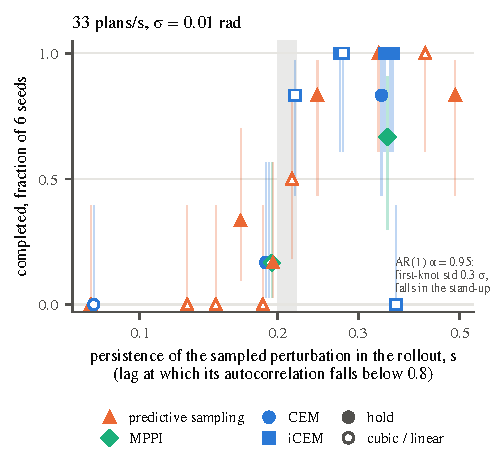
\includegraphics[width=\columnwidth]{figures/planner/fig_persist.pdf}
\caption{\textbf{What the spline changes.} Completion at 33 plans/s and
$0.01$\,rad against the persistence of the sampled perturbation of the
executed action (the lag at which its autocorrelation over the rollout falls
below $0.8$, computed with MJPC's interpolation rules) for twenty spline,
knot-count and noise-colour configurations of PS ($\blacktriangle$), MPPI
($\blacklozenge$), CEM ($\bullet$) and iCEM ($\blacksquare$); hold filled,
cubic or linear hollow. The one point off the step, iCEM with AR(1)
$\alpha=0.95$, fails for amplitude (its first-knot std is $0.3\sigma$).}
\label{fig:planner_persist}
\end{figure}

\begin{figure*}[t]
\centering
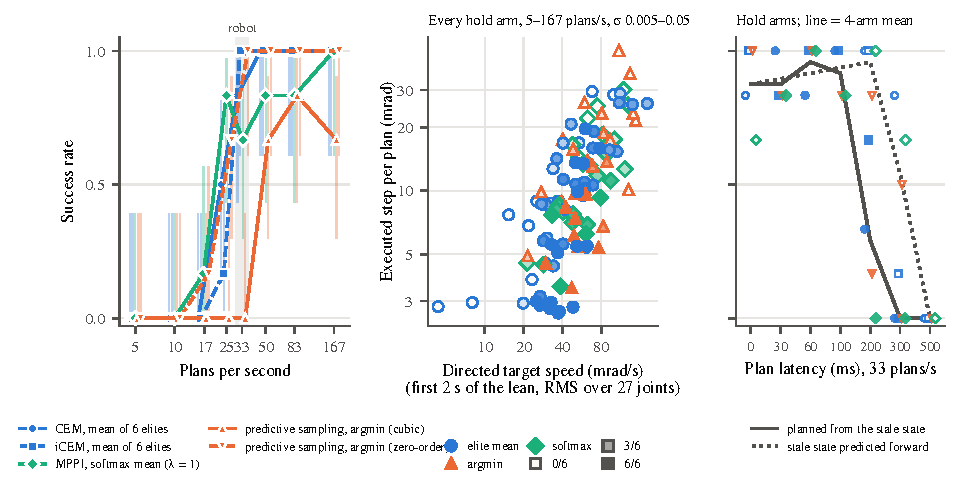
\includegraphics[width=\textwidth]{figures/planner/fig_floor2.pdf}
\caption{\textbf{Plan rate, setpoint speed and latency.} (a) Completion
against plans per second from 5 to 167 for the five update-rule$\times$spline
combinations at $0.01$\,rad; the robot runs at 33. (b) Every hold
configuration at every rate and noise, placed by the directed speed of its
position targets over the first $2$\,s of the lean and by its executed step
per plan; fill is the completion fraction. (c) Completion at 33 plans/s
against plan latency, planned from the stale state (solid) and from the stale
state predicted forward as the deploy node does (dotted).}
\label{fig:planner_floor}
\end{figure*}

%%%%%%%%%%%%%%%%%%%%%%%%%%%%%%%%%%%%%%%%%%%%%%%%%%%%%%%%%%%%%%%%%%%%%%%%%%%%%%%
%% 4. Feedback on main (9).tex (not for the paper; delete)
%%%%%%%%%%%%%%%%%%%%%%%%%%%%%%%%%%%%%%%%%%%%%%%%%%%%%%%%%%%%%%%%%%%%%%%%%%%%%%%
% Dangling / mislabelled references
%  - Methods refers to Sec.~\ref{sec:planner_ablation}; no such label exists.
%    Section 1 above supplies it. The existing "Planner and Cost Ablation"
%    subsection is labelled app:brace_ablation and covers only the brace cost;
%    rename it "Brace-Cost Ablation" and give it its own label.
%  - \label{fig:planners} is a figure with an empty caption
%    (figures/pics/planners_detailed.png); replace with fig_ladder above.
%  - \subsection{Failure Analysis}\label{fig:failure} is referenced as
%    "Sec.~\ref{fig:failure}"; relabel sec:failure.
%  - fig:parameterization (strat11_grid3_topdown_runs.png) has an empty
%    caption; it is the commandability experiment and needs one.
%
% Numbers and consistency
%  - Table tab:planners: "sigma = 8" and "10 rollouts" for PS do not match the
%    deployed task (sampling_exploration 0.12 x half ctrlrange, 20 rollouts);
%    "elite cov." is a diagonal variance with a 0.01 rad floor. See the
%    replacement table.
%  - "The framework uses iLQG ... at 20-50 Hz" (MuJoCo MPC paragraph)
%    describes MJPC's headline planner, not the one deployed here; since the
%    deployed controller is CEM at 33 plans/s, say so in the same sentence or
%    move iLQG to the related-work list.
%  - Task Formulation: "22 Hz planning and increased failure" on the i7 is
%    now explained (Discussion paragraph above): at 0.01 rad the floor is
%    25-33 plans/s.
%  - Leaning, Reaching, and Recovering: "(16/20)$80 \pm 18$\% success (16/20)"
%    duplicates the count; "$100\pm 11$\%" cannot have a symmetric +-11 at
%    100% (Wilson upper bound is 1.0).
%  - Estimation paragraph: "$+267$,mm/min", "$0.48$,m", "$2$,min", "$+210$,mm",
%    "$1$--$2$,mm", "$14$--$47$,mm", "$7$--$10$,mm/s", "$<0.3$,mm" -- the
%    thin-space macro is missing its backslash (should be $267$\,mm/min etc.);
%    same in Target Position Accuracy ("$0.55$,m", "$0.16$,m", "$2.8 \pm 1.3$,cm"
%    ...) and in the fig:target caption.
%  - Abstract says "73% success" for sim-to-real; the body reports 80% on the
%    targeted reach and 73% on max reach -- fine, but say "up to 80%" or name
%    the task in the abstract.
%  - Estimator section: "During such a stand the base genuinely sways, so
%    reported base translation no longer isolates error. Since the base
%    naturally sways during the stand, base translation alone cannot
%    distinguish estimator drift from actual motion." says the same thing
%    twice.
%
% The commandability experiment (Sec. sec:icra, strategy 11)
%  - The bench can give a simulation counterpart on strategy 25's 3x3 target
%    grid (target_col_x / target_col_y numerics) for the four planners; that
%    sweep is running as this file is written (runs/grid_spp15, 3 seeds per
%    cell) and will be reported on the study page. On hardware the natural
%    planner-side statement is that the elite mean's sigma basin (Fig.
%    fig:planner_basin) is what makes one set of weights hold across targets
%    and heights without retuning; the sim grid tests that.
%  - The one model parameter the controller is exposed to is mass (a 10%
%    heavier plant halves completion without gravity feedforward); if the
%    height/target grid carries a payload, say what the payload is relative
%    to the model.
 after the brace-cost ablation, or paste the
% pieces. The section is written to fit in ~0.9 column with one column figure
% (fig_ladder) and one column figure (fig_basin); fig_persist and fig_floor2 are
% offered as appendix figures. Delete the paragraphs marked OPTIONAL to shorten.

%%%%%%%%%%%%%%%%%%%%%%%%%%%%%%%%%%%%%%%%%%%%%%%%%%%%%%%%%%%%%%%%%%%%%%%%%%%%%%%
%% 1. The planner ablation section
%%%%%%%%%%%%%%%%%%%%%%%%%%%%%%%%%%%%%%%%%%%%%%%%%%%%%%%%%%%%%%%%%%%%%%%%%%%%%%%

\begin{figure}[t]
\centering
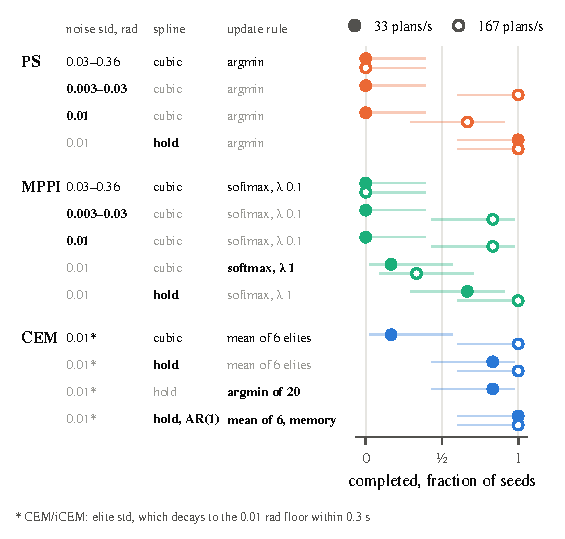
\includegraphics[width=\columnwidth]{figures/planner/fig_ladder.pdf}
\caption{\textbf{From predictive sampling to CEM one component at a time.}
Each row is one planner configuration; in each row the component that changed
from the row above is set in black. Markers show the fraction of six seeds that
completed the lean--reach--recover ladder in simulation at the robot's 33
plans/s (filled) and at 167 plans/s (hollow), with Wilson 95\% intervals.
$0.01^*$: CEM and iCEM sample with the elite standard deviation, which reaches
the $0.01$\,rad floor within $0.3$\,s.}
\label{fig:planner_ladder}
\end{figure}

\subsection{Planner Ablation}\label{sec:planner_ablation}
We compare CEM against predictive sampling (PS) and MPPI on the full ladder
(stand, lean, reach, release, four stand-back rungs) in simulation, on the
robot's joint gains, at the robot's median plan rate of 33 plans/s, six seeds
per configuration (Fig.~\ref{fig:planner_ladder}). As shipped in MJPC, CEM
completes 5/6 and iCEM 6/6; PS and MPPI complete 0/6: PS falls during the initial stand on five of six
seeds (at 4.5--9.9\,s) and collapses onto the table on the sixth, MPPI falls or
collapses before or during the lean on every seed. Two of the three components that differ
between the planners account for the gap, and the update rule
(\textsc{Fold} in Alg.~\ref{alg:skeleton}) is not one of them.

\paragraph{Noise units} CEM and iCEM sample in radians with a $0.01$\,rad
floor. PS and MPPI scale their noise by the actuator control range,
$0.12\times\tfrac12\,\mathrm{ctrlrange}=0.03$--$0.36$\,rad per joint
(median $0.21$\,rad), and drive the position servos with $70$--$130$\,mrad
target steps per plan. Set to $0.01$\,rad in the same units, PS and MPPI
still fail at 33 plans/s (0/6, 1/6) on the cubic spline MJPC's sampling
planner ships with.

\paragraph{Policy representation} With the zero-order hold that CEM and
iCEM hard-code, PS at $0.01$\,rad completes 6/6 and MPPI 4--6/6; with the
cubic spline, CEM itself drops to 1/6. Across twenty spline, knot-count and
noise-colour configurations the separating quantity is how long the sampled
perturbation of the executed action persists in the rollout: every
configuration in which its autocorrelation falls below $0.8$ within
$0.20$\,s completes 0--2/6 and every one that holds it to $0.22$\,s completes
5--6/6, for all four planners (App.~Fig.~\ref{fig:planner_persist}). A hold
with three knots does this by construction ($0.33$\,s); iCEM's AR(1) knot noise
does it by correlation, which is why iCEM alone completes 6/6 with either
spline; white-noise cubic and linear splines do not. At 167 plans/s the
threshold moves below $0.13$\,s and every representation completes.

\paragraph{Update rule} With the hold and $0.01$\,rad every rule completes
the task: argmin (PS, and CEM with one elite) 5--6/6, mean of the $k$ best
5--6/6 for $k\in\{1,2,6,10\}$ and 0/6 for $k=20$ (no selection), softmax
mean 6/6 at $\lambda=0.1$ and 4/6 at $\lambda=1$. The rule decides
sensitivity instead (Fig.~\ref{fig:planner_basin}). Over the twenty
$\sigma\times$plan-rate cells ($\sigma\in\{0.005,\dots,0.05\}$\,rad at 25,
33, 50 and 167 plans/s), CEM completes $\ge 4/6$ in 16, PS with the hold in
12, MPPI with the hold in 10, and PS with its shipped cubic spline in 5; at
33 plans/s CEM's admissible $\sigma$ spans the full tested decade and the
other rules' one octave. The elite mean's random step is $\sigma/\sqrt{k}$
where the argmin's is a full $\sigma$, and that is what lets CEM trade
noise for rate: raising $\sigma$ to $0.02$\,rad takes CEM to 5/6 at
16.7 plans/s and iCEM at $0.03$\,rad to 4/6 at 10 plans/s, where PS and
MPPI gain nothing from the same change.

\begin{figure}[t]
\centering
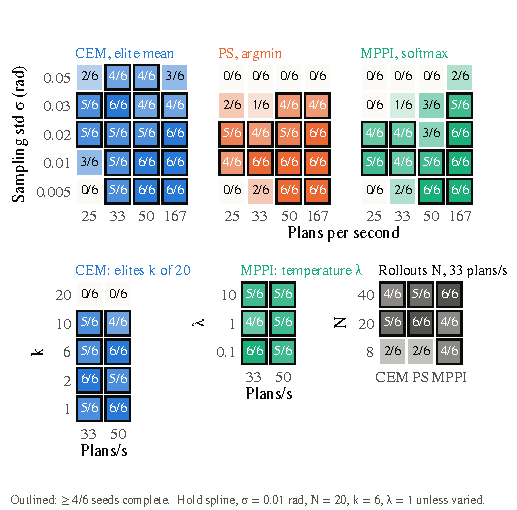
\includegraphics[width=\columnwidth]{figures/planner/fig_basin.pdf}
\caption{\textbf{Sensitivity to configuration.} Completion fraction (6 seeds
per cell) over sampling standard deviation and plan rate for each update
rule at the hold spline; cells at $\ge 4/6$ are outlined. Below: CEM's elite
count, MPPI's temperature, and the rollout count at 33 plans/s.}
\label{fig:planner_basin}
\end{figure}

\paragraph{Plan rate and latency} % OPTIONAL if space is short; the Discussion paragraph below carries the point
At $0.01$\,rad the floor is close to the robot's rate: 25 plans/s completes
1--5/6, 16.7 plans/s 0--1/6, and 10 plans/s 0/6, every failure a backward
fall 2--3\,s into the lean, while the 12\,s stand survives at 5 plans/s. The
executed target step per plan is set by $\sigma$ and the rule, not the rate
(CEM $5$--$8$\,mrad from 167 down to 5 plans/s), so the speed at which the
planner can move its setpoints is step\,$\times$\,rate, and the lean onset
needs $30$--$40$\,mrad/s of directed setpoint motion, which 33 plans/s just
supplies. Latency is a separate quantity: planning
from a state $100$\,ms stale costs nothing at 33 plans/s, $200$\,ms costs
2--5 seeds, and with the state predicted forward as the deploy node does
$200$\,ms costs nothing and $300$\,ms 1--5 seeds. Halving the horizon to
$0.5$\,s completes 0/6, quartering the rollouts 0--2/6, and doubling the
rollout step to $20$\,ms 1--3/6, so the deployed $1$\,s, 20-rollout, $10$\,ms
configuration is close to minimal in every direction but the noise.

\paragraph{Where the rules differ when all complete} % OPTIONAL
The reach rung takes CEM $3.7$\,s, iCEM $4.3$, PS $5.8$ and MPPI
($\lambda=1$) $6.8$\,s, and CEM with six elites braces lightest (peak
$50$\,N, 2\% of the reach on the trunk contact) where PS and MPPI rest on the
table ($138$--$154$\,N, 38--47\%). Under a plant $10\%$ heavier than the
planner's model CEM keeps 3/6 and PS 0/6; under a plant twice as stiff CEM
keeps 6/6, iCEM 4/6, PS 3/6 and MPPI 2/6.

%%%%%%%%%%%%%%%%%%%%%%%%%%%%%%%%%%%%%%%%%%%%%%%%%%%%%%%%%%%%%%%%%%%%%%%%%%%%%%%
%% 2. Replacement for Table~\ref{tab:planners} (the minipage in Methods)
%%%%%%%%%%%%%%%%%%%%%%%%%%%%%%%%%%%%%%%%%%%%%%%%%%%%%%%%%%%%%%%%%%%%%%%%%%%%%%%
% The current table says PS: sigma = 8, argmin, 10 rollouts; CEM: elite cov.
% In this fork every sampling planner reads sampling_trajectories = 20 from
% the task XML, CEM's covariance is diagonal (a per-parameter variance with a
% floor), and PS's sigma is 0.12 x half the control range. Suggested rows:

\refstepcounter{table}
\captionof*{table}{\textbf{Table \thetable.}
How the planners instantiate Alg.~\ref{alg:skeleton} in the deployed
configuration (20 rollouts, 3 spline knots over $1$\,s, a plan every
$30$\,ms). $\sigma$ is the per-knot, per-actuator sampling standard deviation.}
\label{tab:planners}
\centering
\small
\setlength{\tabcolsep}{3pt}
\begin{tabular}{@{}lllll@{}}
\toprule
Planner & \textsc{Center} & \textsc{Spread} & \textsc{Fold} & Spline \\
\midrule
Predictive sampling & $\theta$ (kept as a candidate) & $\sigma = 0.12\cdot\tfrac12\,\mathrm{ctrlrange}$, white & $\arg\min_k J$ & cubic \\
MPPI                & $\theta$ & same as PS & $\sum_k w_k\theta^{(k)},\ w_k\propto e^{-J_k/\lambda}$ & cubic \\
CEM (deployed)      & elite mean & $\max(\text{elite std},\,0.01\,\mathrm{rad})$, diag., white & mean of 6 elites & hold \\
iCEM                & elite mean, 2 elites kept & as CEM, AR(1) across knots ($\alpha=0.7$) & mean of 6 elites & hold \\
\bottomrule
\end{tabular}

%%%%%%%%%%%%%%%%%%%%%%%%%%%%%%%%%%%%%%%%%%%%%%%%%%%%%%%%%%%%%%%%%%%%%%%%%%%%%%%
%% 3. Discussion paragraph: why 33 plans/s is enough
%%%%%%%%%%%%%%%%%%%%%%%%%%%%%%%%%%%%%%%%%%%%%%%%%%%%%%%%%%%%%%%%%%%%%%%%%%%%%%%
% Suggested placement: Sec.~\ref{sec:discussion}, after the first paragraph.
% It also explains the "22 Hz desktop ... increased failure" remark in Task
% Formulation, which the bench reproduces (25 plans/s: CEM 3/6; 16.7: 0/6).

\paragraph{Why 33 plans/s suffices}
Whole-body MPC for locomotion is typically run at 50--100 plans/s over a
300\,Hz tracking controller, because the plan has to re-decide a contact set
every $\approx 0.3$\,s of stance and stabilise an underactuated phase whose
time constant is the pendulum's, $\sqrt{l/g}\approx 0.3$\,s. Supported
reaching has a fixed contact set (double support, then a tripod with the
forearm), a posture the $500$\,Hz joint PD holds between plans, and a single
fast event, the lean onset, that requires the planner to move its position
setpoints at $30$--$40$\,mrad/s (RMS over the 27 joints). A sampling planner moves the setpoints by
roughly one step per plan, so its setpoint speed is step\,$\times$\,rate; at
33 plans/s and $5$--$8$\,mrad per step that is $\approx 190$--$280$\,mrad/s of
executed motion, of which the directed part is enough, and at the 22 plans/s of
the desktop it is not (in simulation CEM completes 3/6 at 25 plans/s and 0/6 at
16.7). The planner here is a setpoint optimiser over a stabilised plant, and
its rate requirement is set by how fast the setpoints have to move, not by the
plant's time constants; a larger sampling step buys back rate, which only the
elite-mean update tolerates.

%%%%%%%%%%%%%%%%%%%%%%%%%%%%%%%%%%%%%%%%%%%%%%%%%%%%%%%%%%%%%%%%%%%%%%%%%%%%%%%
%% Appendix figures (optional)
%%%%%%%%%%%%%%%%%%%%%%%%%%%%%%%%%%%%%%%%%%%%%%%%%%%%%%%%%%%%%%%%%%%%%%%%%%%%%%%

\begin{figure}[t]
\centering
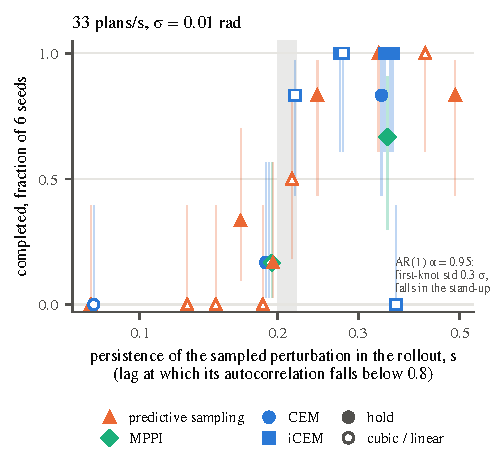
\includegraphics[width=\columnwidth]{figures/planner/fig_persist.pdf}
\caption{\textbf{What the spline changes.} Completion at 33 plans/s and
$0.01$\,rad against the persistence of the sampled perturbation of the
executed action (the lag at which its autocorrelation over the rollout falls
below $0.8$, computed with MJPC's interpolation rules) for twenty spline,
knot-count and noise-colour configurations of PS ($\blacktriangle$), MPPI
($\blacklozenge$), CEM ($\bullet$) and iCEM ($\blacksquare$); hold filled,
cubic or linear hollow. The one point off the step, iCEM with AR(1)
$\alpha=0.95$, fails for amplitude (its first-knot std is $0.3\sigma$).}
\label{fig:planner_persist}
\end{figure}

\begin{figure*}[t]
\centering
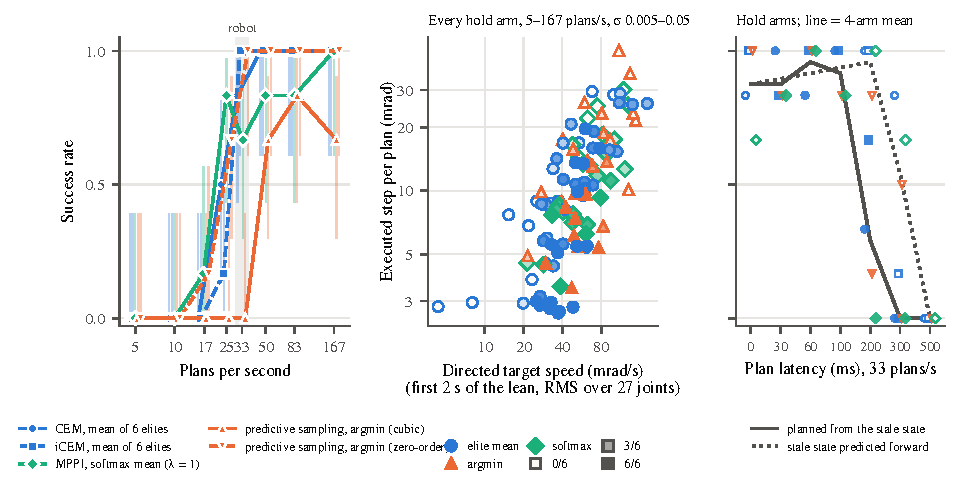
\includegraphics[width=\textwidth]{figures/planner/fig_floor2.pdf}
\caption{\textbf{Plan rate, setpoint speed and latency.} (a) Completion
against plans per second from 5 to 167 for the five update-rule$\times$spline
combinations at $0.01$\,rad; the robot runs at 33. (b) Every hold
configuration at every rate and noise, placed by the directed speed of its
position targets over the first $2$\,s of the lean and by its executed step
per plan; fill is the completion fraction. (c) Completion at 33 plans/s
against plan latency, planned from the stale state (solid) and from the stale
state predicted forward as the deploy node does (dotted).}
\label{fig:planner_floor}
\end{figure*}

%%%%%%%%%%%%%%%%%%%%%%%%%%%%%%%%%%%%%%%%%%%%%%%%%%%%%%%%%%%%%%%%%%%%%%%%%%%%%%%
%% 4. Feedback on main (9).tex (not for the paper; delete)
%%%%%%%%%%%%%%%%%%%%%%%%%%%%%%%%%%%%%%%%%%%%%%%%%%%%%%%%%%%%%%%%%%%%%%%%%%%%%%%
% Dangling / mislabelled references
%  - Methods refers to Sec.~\ref{sec:planner_ablation}; no such label exists.
%    Section 1 above supplies it. The existing "Planner and Cost Ablation"
%    subsection is labelled app:brace_ablation and covers only the brace cost;
%    rename it "Brace-Cost Ablation" and give it its own label.
%  - \label{fig:planners} is a figure with an empty caption
%    (figures/pics/planners_detailed.png); replace with fig_ladder above.
%  - \subsection{Failure Analysis}\label{fig:failure} is referenced as
%    "Sec.~\ref{fig:failure}"; relabel sec:failure.
%  - fig:parameterization (strat11_grid3_topdown_runs.png) has an empty
%    caption; it is the commandability experiment and needs one.
%
% Numbers and consistency
%  - Table tab:planners: "sigma = 8" and "10 rollouts" for PS do not match the
%    deployed task (sampling_exploration 0.12 x half ctrlrange, 20 rollouts);
%    "elite cov." is a diagonal variance with a 0.01 rad floor. See the
%    replacement table.
%  - "The framework uses iLQG ... at 20-50 Hz" (MuJoCo MPC paragraph)
%    describes MJPC's headline planner, not the one deployed here; since the
%    deployed controller is CEM at 33 plans/s, say so in the same sentence or
%    move iLQG to the related-work list.
%  - Task Formulation: "22 Hz planning and increased failure" on the i7 is
%    now explained (Discussion paragraph above): at 0.01 rad the floor is
%    25-33 plans/s.
%  - Leaning, Reaching, and Recovering: "(16/20)$80 \pm 18$\% success (16/20)"
%    duplicates the count; "$100\pm 11$\%" cannot have a symmetric +-11 at
%    100% (Wilson upper bound is 1.0).
%  - Estimation paragraph: "$+267$,mm/min", "$0.48$,m", "$2$,min", "$+210$,mm",
%    "$1$--$2$,mm", "$14$--$47$,mm", "$7$--$10$,mm/s", "$<0.3$,mm" -- the
%    thin-space macro is missing its backslash (should be $267$\,mm/min etc.);
%    same in Target Position Accuracy ("$0.55$,m", "$0.16$,m", "$2.8 \pm 1.3$,cm"
%    ...) and in the fig:target caption.
%  - Abstract says "73% success" for sim-to-real; the body reports 80% on the
%    targeted reach and 73% on max reach -- fine, but say "up to 80%" or name
%    the task in the abstract.
%  - Estimator section: "During such a stand the base genuinely sways, so
%    reported base translation no longer isolates error. Since the base
%    naturally sways during the stand, base translation alone cannot
%    distinguish estimator drift from actual motion." says the same thing
%    twice.
%
% The commandability experiment (Sec. sec:icra, strategy 11)
%  - The bench can give a simulation counterpart on strategy 25's 3x3 target
%    grid (target_col_x / target_col_y numerics) for the four planners; that
%    sweep is running as this file is written (runs/grid_spp15, 3 seeds per
%    cell) and will be reported on the study page. On hardware the natural
%    planner-side statement is that the elite mean's sigma basin (Fig.
%    fig:planner_basin) is what makes one set of weights hold across targets
%    and heights without retuning; the sim grid tests that.
%  - The one model parameter the controller is exposed to is mass (a 10%
%    heavier plant halves completion without gravity feedforward); if the
%    height/target grid carries a payload, say what the payload is relative
%    to the model.
